%\documentclass[12pt,twocolumn]{article}
\documentclass[10pt, conference, compsocconf]{IEEEtran}

%\usepackage{url}
\usepackage{graphicx}
\usepackage{hyperref}
%\usepackage[small,bf]{caption}
\usepackage{balance}

\title{SECR3T: Secure End-to-End Communication over 3G Telecommunication Networks}

%\author{G. Cattaneo, G. De Maio, F. Petagna\\
%Dipartimento di Informatica e Applicazioni ``R.M. Capocelli"\\
%Universit\`a di Salerno\\
%{\{cattaneo, gdemaio, fabpet\}@dia.unisa.it}\\
%}

\author{
  \IEEEauthorblockN{
    Giuseppe Cattaneo%\IEEEauthorrefmark{1}
    , Giancarlo De Maio%\IEEEauthorrefmark{2}
    , Fabio Petagna%\IEEEauthorrefmark{3}
  }
  \IEEEauthorblockA{
    Universit\'a di Salerno\\
    Dipartimento di Informatica e Applicazioni\\
    cattaneo@dia.unisa.it%\IEEEauthorrefmark{1}, 
    , g.demaio@gmail.com%\IEEEauthorrefmark{2}, 
    , fabpet@dia.unisa.it%\IEEEauthorrefmark{3}
  }
}

%\date{\today}

\begin{document}

\maketitle

\begin{abstract}

Nowadays the use of video conference tools from mobile devices is becoming more widespread. Unfortunately, solutions based only on the security features inherited from the operator infrastructure cannot be blindly trusted. Therefore, the need for secure communication tools is rapidly increasing.
%In order to save time and pollution to the planet, many managers could be interested in participating in virtual business meetings whereas the video call tool could be proved to be reliable enough both for privacy and effectiveness.
Currently, voice and video communication tools are considered unreliable when used in either a mobile context or under poor signal strength conditions. This is particularly true for IP connections routed on the Packet-Switched Domain (PSD) over 3G mobile networks.

%This project aimed to give a solution to handle the lack of  communication tools explicitly designed to increase the security level over the Circuit-Switched Domain (CSD) of 3G networks.
This paper presents the design and the implementation of SECR3T (Secure End-to-End Communication over 3G Telecommunication Networks), a fully-fledged secure communication system for mobile devices based on the native Circuit-Switched Domain (CSD) of 3G networks.
%At our knowledge do not exist solutions addressing the communication security over the CSD of 3G networks.
%At our knowledge this last feature is the most innovative contribute of the project.
To the authors knowledge, this is the first solution for secure communication over the CSD of 3G networks.

The security schemes implemented by SECR3T include mutual end-to-end authentication as well as data encryption. The adopted end-to-end security mechanisms have been embedded within the native 3G-324M protocol and do not require any form of interaction with the mobile network operator.

Relying on the CSD, SECR3T provides a better QoS with respect to the PSD based solutions for 3G networks. It also requires less power consumption as the user is registered once on the Base Station (BS), with the handset not having to implement any heavy keep-alive protocols.
In order to prove the effectiveness of the adopted strategy, a prototype was implemented to compare its performance with the well-known PSD solutions. Subsequently, the authors experimentally evaluated the security strengths and the impacts produced on the user experience with respect to traditional tools using CSD.

%SECR3T has been extensively tested in critical environments such as business meeting and on-line trading and in many cases it gave better performance with respect to the IP-based tools. This was due to the use of lines affected by a high BER value, as typically happens in rural areas with low signal coverage.

%Through an accurate experimental analysis we demonstrated that the extensions to the original protocol we propose do not significantly affect the user expected performances. Moreover, as proof of concept the paper shows how a device equipped with SECR3T is able to transparently interoperate with standard devices.

%Questo lavoro presenta una full size implementatiotion di un sistema di videoconferenza sicura usato per valutare e dimostrare sperimentalmente che
\end{abstract}

\begin{IEEEkeywords}
UMTS; 3G-324M; X.509; mobile; CSD; audio/video; encryption; power consumption.

\end{IEEEkeywords}

\section{Introduction}
\label{par:intro}

%Public and private sectors extensively rely on 3G mobile networks for communicating sensitive, technical, financial, political and personal information. Videoconference is a service increasingly used for business and top-management affairs. A reliable videoconference service might be available always and everywhere. For example, a company manager might be able to perform a business videoconference in high-mobility environments as traveling by train or in isolated places as staying on boat quite far from the coast.
%3G mobile networks provide circuit-switched channels with bandwidth and QoS constraints which cannot always be satisfied by IP-based connections in relation to reachability and availability requirements.

The services provided by modern 3G telecommunication technology can be divided into two classes, each in charge of two different network domains: Circuit-Switched (CS) and Packet-Switched (PS) domain. Different domains provide different services, for example, videotelephony is routed to the CS domain while IP networking takes place in the PS domain.

Unlike IP networks, terminals in 3G networks are not affected by addressing problems. Every device equipped with an USIM is automatically connected to the mobile network and made available through its telephone number to other mobile devices. Moreover, UMTS networks provide an adequate QoS for real-time communications, including minimum cell rate (64Kb/sec for video-calls) and low latency. The CS connection between terminals is carried out and managed by the network.
%, simplifying the videotelephony application structure.

%Mobile networks are part of everyday life, thanks to third-generation (3G) mobile networks users can be connected to the Internet at anytime and anyplace using mobile devices such as smartphones, laptops and netbooks.
%Public and private sectors extensively rely upon 3G mobile networks for communicating sensitive technical, financial, political and personal information.
Telecommunication companies have put a great deal of effort into the diffusing, global coverage and amount of different services provided to the users, such as videotelephony, text messaging and data communication. However, less effort has been put into providing suitable end-to-end security mechanisms for these services. In fact, voice, text and video communications carried out using 3G networks have been proven to be vulnerable to eavesdropping and unauthorized access. Both wireless data links as well as wired parts of the network are susceptible to several security threats.

% Services provided by the modern third-generation (3G) telecommunication technology can be split into two classes, each in charge of two different network domains: Circuit-Switched (CS) and Packet-Switched (PS) domain. Different domains provide different services, for example, videotelephony is routed to the CS domain while IP networking take place in the PS domain.

%3G mobile networks allow the users to hold a voice call while surfing the internet because the core of network is split into two main domains, the Circuit-Switched domain (CS) and the Packet-Switched domain (PS)\cite{umtsbook}. Different domains provide different services, for example, videotelephony is routed to the CS domain while IP networking take place in the PS domain.

%Very often the telecommunication infrastructure provide an optimal signal strength and very good communication quality for traditional audio and audio/video communication services (routed through the CS domain) but poor quality for IP-based services (routed through the PS domain).

%An important factor which can affect IP communications in 3G mobile networks is the hight Bit Error Rate (BER) of the wireless links. On the other hand, in the CS domain, network communication protocols where expressly designed to overcome the problems caused by the hight BER (see Section \ref{3G324M}).

%This work presents a specific solution for secure video-calling over the CS domain, but also is a starting point to experiment similar systems for other 3G services.

%Due to these considerations, it seems obvious that end-to-end mechanisms for secure audio, video and text communications over 3G mobile networks are needed.

%As long as videotelephony is essentially a data communication, both CS and PS domains on the 3G networks are suitable for this service. The adoption of the PS has many advantages but also some important drawbacks with respect to the CS. The biggest advantage consists in the use of the IP protocol  which ensure interoperability with almost all network applications for both mobiles and desktops. Moreover, IP security protocols such as SSL, IPSEC and VPN, and already designed systems for end-to-end security at application level can be re-used almost without modifications. Even if, effective and easy-to-use solutions have been presented for voice/video communications over IP networks, an effective and reliable videotelephony service have reachability and availability requirements which can't be always satisfied by an IP-based mobile network. To be able to begin or receive a call the device must be always connected to the network. In mobile IP network this means that the mobile device must establish a connection in the PC domain of the 3G network and maintain this IP connection allays on. As long as the the mobile networks have not a global coverage, handover processes tends to make the channel unstable and computational effort to maintain an IP connection may greatly reduce the device autonomy due to the battery discharge. On the contrary, the CS network connection are more stable in high-mobility environments and less battery consuming, there is no need to maintain any other communication channel other than the one with the network carrier. An other important factor which can affect IP communications in 3G network is the hight Bit Error Rate (BER) of this network. While in the CS domain network communication protocols where expressly designed to overcome the problems caused by the hight BER (see Section \ref{3G324M}), PC communication protocols were designed for more stable communication channels.

Considering that videotelephony is essentially ``data communication'', both CS and PS domains on the 3G networks are suitable for this service. The adoption of the PS has many advantages but also several relevant drawbacks with respect to the CS. The most significant advantage of the PSD is the use of the IP protocol, which ensures interoperability with almost all network applications for both mobile and desktop devices. IP security protocols such as TLS, IPSEC and VPN, along with already existing systems for end-to-end security at application level, can be reused  without any modifications.
Even if efficient and easy-to-use solutions have been presented for voice/video communications over IP networks, an effective and reliable videotelephony service needs both reachability as well as availability which cannot be always satisfied by an IP-based mobile network. Given that mobile networks do not have global coverage, handover processes and high Bit Error Rate (BER) on the wireless link tend to make the channel unstable. On the contrary, the CS network connections are more stable in high-mobility and high-BER conditions, thus granting reachability and availability %requirements
to the users.

In this work, a metric to evaluate the communication service, based on the following key performance indicators, has been defined: voice and video quality, user data privacy and application impact on the battery life. These metrics are often related to the domain that provides the service. Generally, videotelephony over the CS domain results in a better quality and greater battery saving with respect to the PS domain. In fact, the CS connections between the endpoints are provided by the telecommunication network with a higher QoS value, with it being managed by the BSs rather than by the IP connections which are managed by the peers. On the contrary, applications running over the CS domain must comply with inflexible network protocols through which it is hard to provide the same security level of the applications running over IP.
%the tradeoff "quality/security" hangs on the left side in the case of videotelephony over CS domain, on the right side in the case of videotelephony over PS domain.
The aim of this work is to improve the security of videotelephony over the CSD, in order to achieve an optimal trade-off for the key performance indicators discussed above.

%This paper proposes an alternative to IP-based systems for secure voice and video communication in the CS domain of 3G mobile networks. CS domain is a network infrastructure for conversational multimedia based services which PS wireless networks cannot deliver because of inherent IP traffic overhead, BER sensitivity, and variant routing delays.

\subsection{Trusting}

When an end-user signs a cell-phone contract, he implicitly trusts the mobile network operator, which is supposed to preserve communication privacy. Therefore, the mobile network operator must guarantee adequate security measures to accomplish this task. While on 3G mobile networks, channel encryption has been adopted for wireless links, user data on wired links is transmitted in clear, thus introducing several potential threats. Moreover, 3G networks extensively rely on roaming, following agreements signed between two or more operators. This means that end-users should also trust the roaming operator, given that the physical telecommunication channel is managed by another company.

%Network and intra-network domain security are actually covered by Mobile Application Part Security (MAPSec)\cite{mapsec} protocol, that provide security support for the MAP\cite{map} protocol. The MAP protocol plays a central role in the signaling communications between the Network Elements (NEs).  User profile exchange, authentication, and mobility management are performed using MAP. MAP typically runs over the Signaling System number 7 (SS7) protocol stack\cite{ss7}. MAPSec protocol protects MAP messages trough a packet-encapsulation mechanism.

%It is important to note that the mobile station is not affected by network domain security. The two communicating NEs may both be in the same network administrated by the same telecommunication operator or they may belong to two different networks administrated by two different companies. Because MAPSec only provides encryption of MAP signalling messages but not user traffic, unauthorized communication interceptions, performed by malicious users who have access to the physical telecommunication infrastructure, are a real threat.
%On the other hand, traffic encryption at network-level would raise intra-network interoperability issues and would require sophisticate mechanisms for interceptions performed by legal authorities (magistrates, security forces etc.).

Encryption at network level may raise several issues. Assuming that end-to-end user communication passes through a lot of network elements, interoperability between different mobile network operators may be harder to reach because cryptographic keys and security protocols should be deployed among network elements managed by different providers. Moreover, there are authorities that must be able to implement phone tapping. In many countries, there are laws against terrorism which enforce the ability of the network operators to intercept the communications related to a suspected user. Encryption at network level may also interfere with these tasks.

%Substantially, user traffic may be transmitted encrypted through all network links and entities to avoid unauthorized interceptions, encryption at network-level may cause administrative issues due to VNOs, and at the same time a third-trusted-part must be able to easily decrypt  communications to allow authorized phone tapping.

The solution proposed in this paper is an end-to-end security mechanism for 3G videotelephony. Such a solution may also include fair mechanisms for key-escrow.


\subsection{Security background}

In 1999, with the standardization process of 3G mobile networks, the 3GPP\footnote{The 3rd Generation Partnership Project (3GPP), \url{http://www.3gpp.org/}} Consortium, which is in charge of producing the technical specifications for the 3G mobile networks, proposed improved security mechanisms for wireless channels with respect to the GSM ones, which have been proven to be vulnerable.
The 3GPP introduced a stronger authentication and key-agreement protocol performed by mobile devices and networks, as well as a stronger cryptosystem for wireless data encryption (A5/3 based on the KASUMI~\cite{kasumi} algorithm). However, effective attacks which can lead to the decryption of the communication channel have been discovered. Keller and Shamir presented an attack on KASUMI which makes it possible to recover a full A5/3 key using a related-key attack~\cite{A53attack}. Karsten et al.~\cite{srsly} showed how to perform a semi-active attack by jamming UMTS frequencies and forcing the mobile device to switch to GSM mode.
%Using the Karsten technique, an attacker can ask the USIM to reuse a previous A5/3 key for a breakable obsolete GSM encryption protocol, as A5/1, and can decrypt a previously intercepted conversation.

%Security of mobile-telephony communications only depends on network-level protocols and assumes the presence of trusted entities in the proprietary network infrastructure, in fact only wireless link is encrypted.
%Network and intra-network domain security are covered by Mobile Application Part Security (MAPSEC)\cite{mapsec} protocol, which only encrypt Mobile Application Part (MAP) signalling messages but not user traffic.
%Whereas for the wireless transport has been adopted channel encryption, all the wired part is still transmitting in clear introducing several threats. In this scenario, unauthorized communications interception performed by malicious users who have access to the physical telecommunication infrastructure is a real problem.
%On the other hand, traffic encryption at network-level would raise intra-network interoperability issues and would require sophisticate mechanisms for interceptions performed by legal authorities (magistrates, security forces etc.).

%Security issues also involves intra-network domain. For example, a Virtual Network Operator (VNO) is a provider of management services and a reseller of network services from other telecommunications suppliers that does not own the telecommunication infrastructure: as the previous case, only MAP signalling messages passing through the hosting network are protected. Trade secrets and other confidential data pass in plain text through competitor networks.

%Securing this information and its transmission as well as the access to the mobile network is necessary for the secure and smooth operation of the system
%Most IP-based telephony protocols provides suitable security measures for user authentication, traffic encryption and data integrity. Otherwise the telecommunication companies never guaranteed  the same security level for communications through their networks.

%Due to these considerations, end-to-end security mechanisms based on fair cryptosystems seems to be the better choice.
There are several projects addressing application-level end-to-end security of voice communications over mobile networks, such as SPEECH~\cite{speech}. To the authors knowledge, there are currently no tools addressing the security of the videotelephony communication routed by the CSD of the 3G mobile networks.

%In the past, the ITU-T H.323 standard has been the most used for videotelephony over packet-switched networks as Internet, and its application-level security concerns are addressed in the ITU-T H.235 recommendation. Even though the H.235 purpose is to address the application-level security of H.3XX family protocol, it is strongly related to H.323 and does not seems to be the better choice for the newer ITU-T H.324M standard, projected for mobile telephony networks.


%In this paper is presented a system which ensures the security of voice and video communication over 3G mobile networks, projected to transparently extent 3G-324M protocol.
%The main goal is the demonstration that it is possible to integrate cryptographic mechanisms within the 3G-324M (and most generally H.324) protocol in a totally transparent way for the telephone company, preserving compatibility with the UMTS specifications and with a very low impact on the system performance.

%The proposed system ensures mutual authentication for the users and key agreement by means of X.509 digital certificates and end-to-end encryption by means of AES for the communication channel.

%The theoretic results was supported by the implementation of a secure videotelephony application prototype including well-known strong cryptographic protocols for user authentication, communication encryption and data integrity, fully compatible with the UMTS specifications. In particular, we projected and realized a general-purpose flexible framework to provide the H.324 standard with the support for security modules. The demonstrable implemented prototype has been successfully tested on personal computers equipped with commonly used UMTS Tokens, and its performance seems to be good enough for a large-scale real implementation.

\subsection{Outline}
The rest of the paper is organized as follows. Section~\ref{par:requirements} presents the requirements of the project. In Section~\ref{par:3G324M}, the 3G-324M communication protocol is described, while in Section~\ref{par:design} the integrations aimed at enhancing the security of the protocol are discussed. In Section~\ref{par:perf}, the impact on the overall system performance is briefly evaluated. The paper ends with a discussion on future studies in Section~\ref{par:future} and the authors conclusions in Section~\ref{par:conclusions}.

\section{Requirements}
\label{par:requirements}
The main aim of this work is to present a system that realizes a secure video-call over 3G mobile networks with the following requirements:
%\begin{itemize}
\begin{list}{\labelitemi}{\leftmargin=1em}
  \item \textit{Strong end-to-end user authentication through digital certificates.}
In order to achieve the strong end-to-end user authentication requirement, it is supposed that the user adopts a X.509 digital certificate issued by a trusted Certification Authority (CA), with it being securely stored on the mobile equipment.
  \item \textit{End-to-end user communication encryption.}
The audio, video and data channel encryption requirements can be achieved by using robust and well-known encryption algorithms. The authentication protocols must also implement key-agreement mechanisms in order to properly initialize the channel encryption.
  \item \textit{Compliance with videotelephony protocols.}
The proposed solution must be compliant with existing applications and not require any modifications to the native videotelephony protocol.
  \item \textit{Infrastructure-side transparency.}
It is required that no extra effort should be made by the network elements to support the described end-to-end security mechanisms, therefore the encrypted data must be transmitted between users as normal network traffic.
  \item \textit{Limited impact on system performance.}
The introduction of security mechanisms should not considerably affect the system performance and the user experience. For example, the initial handshake should not delay the communication longer than a few seconds. Analogously, during the conversation, communication delays due to data encryption should not be longer than 300 milliseconds.
\item \textit{Device constraints.}
In order to cope with the low processing power as well as save battery life, local computations and end-to-end communications must be minimized. The secure video-call system should implement public-key encryption schemes based on the Elliptic Curve Cryptography\footnote{With respect to RSA, ECC offers equivalent security with smaller key sizes, which results in faster computations, lower power consumption as well as memory and bandwidth savings.} (ECC) instead of traditional public-key cryptosystems.
%\end{itemize}
\end{list}

%\section{State of the art}
%\label{art}

%There exists a lot of videotelephony applications implementing security measures, most projected for IP networks. Most telephone companies now also function as internet service providers (ISPs), and the distinction between a telephone company and an ISP may disappear completely over time, as the current trend for supplier convergence in the industry continues. At the same time, recent landline telephones support video calling and conferencing over Internet, using the SIP protocol (or similar) to initialize the call.
%Communications over IP can be encrypted using robust well-known protocols as SSL, IPSec etc., or proprietary algorithms as in the Skype protocol.

%In the first 2000s, the 3GPP corporation standardized the third-generation (3G) mobile telecommunications technology, known as UMTS. Respect to GSM, one of the most important improvement of UMTS is the network support for multimedial communications. 3G-324M is the supported standard for videotelephony, based on ITU-T H.324M recommendation (there are very few differences). Up to this time, a lot of mobile devices are able to run 3G-324M video-calling applications.

%Today, security of mobile-telephony communications only depends on network-level protocols and assumes the presence of trusted entities in the proprietary network infrastructure.
%In the past, the ITU-T H.323 standard has been the most used for videotelephony over packet-switched networks, and its application-level security concerns are addressed in the ITU-T H.235 recommendation. Even though the H.235 purpose is to address the application-level security of H.3XX family protocol, it is strongly related to H.323 and does not seems to be the better choice for the newer ITU-T H.324M standard, projected for mobile telephony networks.

%There exists some projects addressing application-level security of voice communications over mobile-telephony networks, as SPEECH \cite{speech}. However, until this article, it doesn't seem to exist any public research addressing application-level security of \emph{videotelephony} communications over UMTS.

%Breve spiegazione di SPEECH e SPhone4


\section{Videotelephony over UMTS}
\label{par:3G324M}

In this section a brief introduction to the 3G videotelephony protocol is presented in order to explain how it can be extended to support security mechanisms.

3G-324M~\cite{3g324m} is the 3GPP umbrella protocol for videotelephony in 3G mobile networks. The 3G-324M protocol operates over an established CS connection between two communicating peers. It is based on the ITU-T\footnote{International Telecommunication Union - Telecommunication Standardization Sector, \url{http://www.itu.int/ITU-T/}} H.324~\cite{h324} specification for multimedia conferencing over CS networks.

%3G-324M does not support end-to-end encryption but security only depends on network-level protocols in charge of the network.

%3G-324M is a derivative of the existing ITU-T recommendation H.324 for low bit-rate media communication, which was initially intended for videotelephony using modem-based communication over the PSTN.

%One of the key concepts of H.324 is that of logical channels. \emph{Logical channel number 0} (LCN0) is dedicated to control information.

%It is implicitly opened as soon as a connection has been established, using an associated multiplexer frame structure that allows LCN0 information to be transmitted and received.
%Using LCN0 the terminal can immediately start sending and receiving control information following the syntax and semantics defined in ITU-T recommendation H.245, allowing it to declare its capabilities and discover the capabilities of the remote terminal.
%Both terminals then use this information to open additional logical channels that are consistent with the declared capabilities.

%Another key feature is the approach taken to multiplexer frame structures - the way that octets in each frame are allocated to control, media, and data information. Each terminal can have up to 16 multiplexer frame structures. One of these is predefined for use with LCN0 at the start of the session. The structure of the other multiplexer frames that the terminal will use is signaled to the receiving terminal at the start of the session, in the form of \emph{multiplex table entries} (MTEs). There is no requirement for a terminal to send or use all 15 MTEs, and communicating terminals are not restricted to using common set of MTEs.

%H.223 provides the multiplexing function for H.324.
%It has two-layer structure: the upper \emph{adaptation layer} (AL) provides three ways of adapting media, data and control information (known as AL1, AL2, AL3), which provide increasing levels of error protection. The lower multiplexer layer takes information from different sources passed to it by the adaptation layer and combines it to form multiplexer frames. It also performs the reverse operation on incoming frames.

%The \emph{simple retransmission protocol} (SRP) layer between the H.245 control process and the multiplexer is designed to provide reliable, acknowledged transmission of control information.

%The mandatory video codecs for H.324 are H.261 and H.263, and the mandatory audio codec is G.723.1.

%H.324 also covers procedures for interfacing to a synchronous modem and call initiation using the modem, but they are not used in the derived 3G-324M.

%Annex C of H.324 was introduced as a result of studies on how H.324 could be adapted for use over wireless and mobile networks. H.324 with Annex C has become known as H.324M. 3G-324M removes the modem requirements for H.324 and assumes that a transparent digital channel is available.
%Annex C provides enhanced mechanisms for robustly multiplexing and error resilience with respect to H.324. Moreover, it provides enhanced procedures for more reliable delivery of H.245 control messages.
%Annex C provides three possible additional modes for robustly multiplexing information: there are known as mobile levels 1, 2 and 3. Mobile level 0 is the basic mode of operation of the multiplexer in H.324 without Annex C. Annex C of H.324 defines a mobile level detection mechanism to allow terminals to synchronize at the start of a session and establish which of the possible mobile levels is to be used to send multiplexed information. A mechanism for changing mobile level during a session is provided.

%Annex C also provides enhanced procedures for more reliable delivery of H.245 control messages by specifying the use of numbered SRP (NSRP) instead of SRP. A layer known as the \emph{control segmentation and reassembly layer} (CCSRL) is introduced between the H.245 signaling entities and the NSRP layer. The purpose of CCSRL is to segment larger control messages, to reduce the susceptibility of control messages to error.

%The only change to the mandatory codecs is that support for Annex C of G.723.1, "scalable channel coding scheme for wireless applications", is recommended.

%\subsection{3G-324M extension}

\begin{figure}[!htbp]
\centering
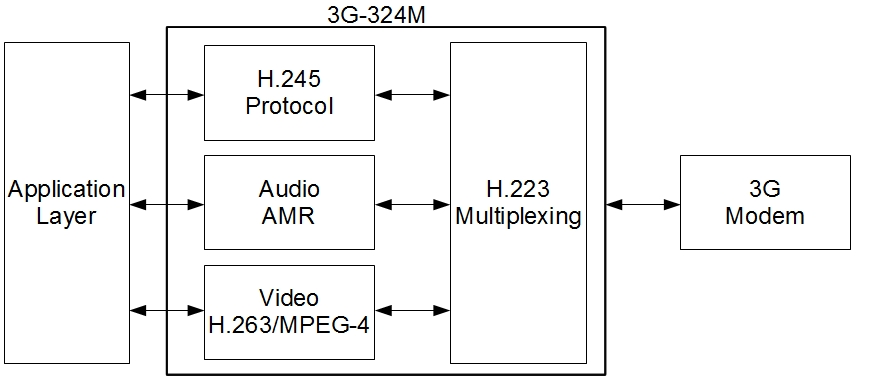
\includegraphics[scale=0.28]{pics/3g324m.jpg}
\caption{3G-324M protocol: simplified architecture.}
\label{fig:3g324}
\end{figure}

%3GPP has taken H.324M as starting point and modified it to create 3G-324M. For Release 99 the principal differences between 3G-324M and H.324M are in the codecs supported.

Figure~\ref{fig:3g324} shows the main components of the 3G-324M protocol. The H.245 protocol is designed to provide reliable, acknowledged transmission of session control information. It uses a Numbered Simple Retransmission Protocol (NSRP) as well as a Control Segmentation and Reassembly Layer (CSRL) in order to segment larger control messages and reduce their susceptibility to error. H.223 provides the functions used to multiplex audio, video and text in a single stream processed by a 3G modem. The audio and video modules provide standard procedures to encode the media streams. The mandatory audio codec for 3G-324M is GSM-AMR~\cite{amr}. H.263~\cite{h.263} is the mandatory video codec whereas the MPEG4 is optional. The Application Layer (AL) represents the existing videotelephony application and is not part of the 3G-324M protocol stack.

%\subsection{3G-324M extension}

%Referencing Figure \ref{fig:3g324sec}, the Application Layer (AL) represents the existing videotelephony application and is not part of the 3G-324M protocol stack.
%%It interacts with the H.245 module which provide the support to set up and manage the call.
%The Security Control Layer (SCL) is a middleware added to provide the AL with the procedures to initialize and manage the security protocols. It uses the reliable H.245 protocol to interact with the peer. The AL also sends to and receives data from the Audio/Video (A/V) modules, which take in charge the communication of the multimedial streams. A/V data can pass trough an Encryption Layer (EL) which provide the encryption functions for the outgoing streams and the decryption functions for the ingoing streams.

%Different priorities and error-resilience strategies are applied to audio, video and control data, . The segmentation and error-resilience procedures run regardless of the packet content. The multiplexing and de-multiplexing procedures are symmetric.

%It is important to note that the proposed extensions do not impact over the existing videotelephony protocol and can be transparently integrated within 3G-324M.

%and in the limiting of mandatory support by the multiplexer to levels 1 and 2. Mobile level 3 is optional: use of this level may make to high computational demand on the handset.

\paragraph{Considerations on the video codecs}
\label{par:videocons}
The video codecs used in the 3G-324M protocol have some characteristics which are to be considered for the correct design of the SECR3T framework.

On the transmitter side, H.263 and MPEG-4 codecs produce variable-length frames which are divided into Group Of Blocks (GOBs) to be sent to the multiplexing level. Every GOB has a resynchronization marker to reduce the error propagation caused by the nature of Variable Length Code (VLC) into a single frame.
%The resynchronization marker is inserted at the top of a new GOB with the header information so that decoding can be done independently.
On the receiver side, the blocks are received one-by-one from the multiplexing layer, with the reception of a resynchronization marker indicating the start of a new GOB.
Due to the resynchronization marker and the VLC, the encryption of a GOB must be performed block-by-block.
%The received GOB is recomposed using the information of its header and is passed to the video codec for the decoding.


\section{A secure video-calling system}
\label{par:design}

%\begin{figure}[!htbp]
%\centering
%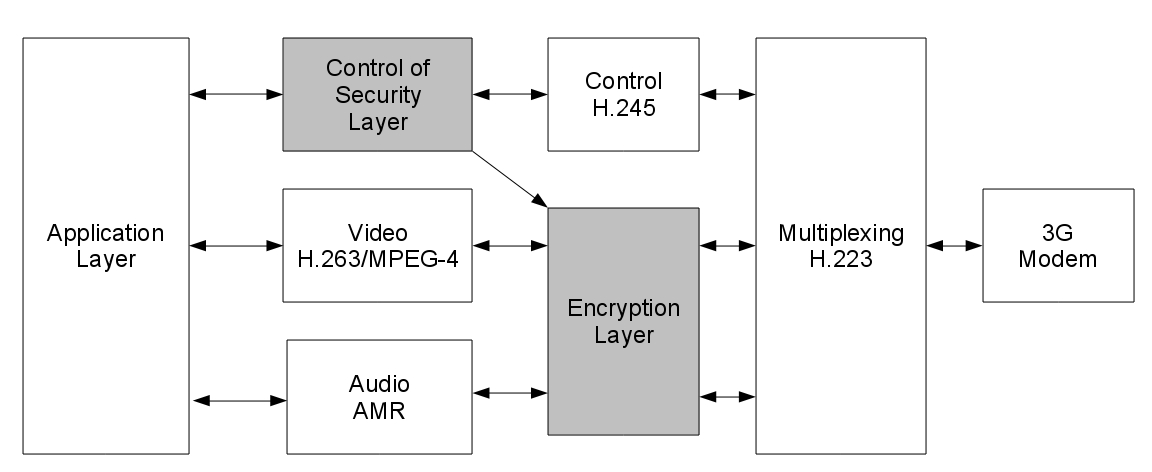
\includegraphics[scale=0.35]{pics/3g324m_template_fmw_bn.jpg}
%\caption{SECR3T high-level architecture}
%\label{fig:3g324sec}
%\end{figure}

\begin{figure}[!htbp]
\centering
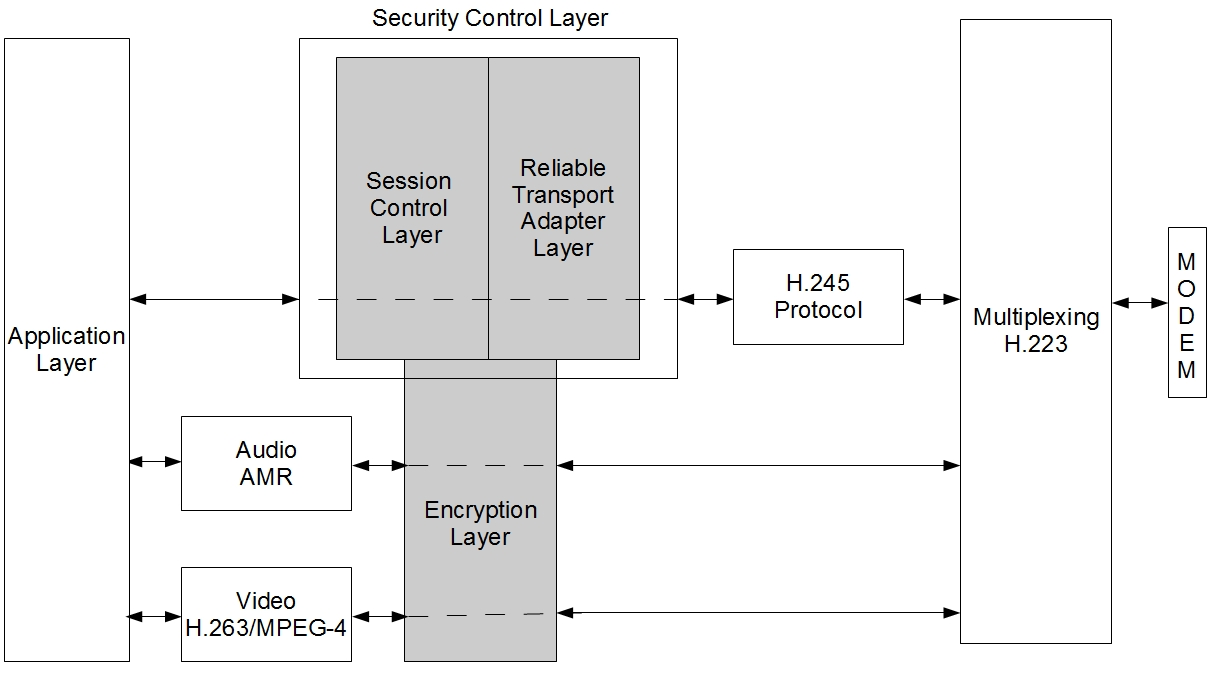
\includegraphics[scale=0.20]{pics/framework_bn.jpg}
\caption{The extended 3G-324M architecture: the white modules compose the original 3G-324M architecture. The gray modules represent the proposed extensions for secure end-to-end communication.}
\label{fig:3g324sec}
\end{figure}

%It interacts with the H.245 module which provide the support to set up and manage the call.

\subsection{High-level design}
\label{par:hlvl}
The SECR3T project consists of a framework which extends the 3G-324M specification and makes it possible to integrate security mechanisms within the existing videotelephony protocol. The high-level architecture of SECR3T is shown in Figure~\ref{fig:3g324sec}.
The Security Control Layer (SCL), which includes the Session Control Layer (SESCL) and the Reliable Transport Adapter Layer (RTAL), is a middleware added to provide the AL with the procedures to initialize and manage the security protocols. It uses the reliable H.245 protocol to interact with the peer. The AL also sends to and receives data from the Audio/Video (A/V) modules, which control the communication of the multimedial streams. A/V data can pass through the Encryption Layer (EL) which provides the encryption functions for the outgoing streams as well as the decryption functions for the incoming streams.

%The white components represent the existing 3G-324M modules, explained in the Section \ref{par:3G324M}, and the grey components are the SECR3T meta-modules.
The SCL implements the configuration module, the key-agreement and authentication protocols. The EL includes the audio, video and text encryption mechanisms.
%SECR3T supports a lot of security-related functions as user authentication through digital certificates, communication encryption and data integrity.

%Using SECR3T, call setup is speed-up as initialized by 3G-324M protocol, and the stable dedicated circuit-switched connection is established between the users at the expense of the network. %and is not part of the 3G-324M protocol.

%This paper shows as 3G-324M protocol can be extended to support a lot of security-related functions as user authentication through digital certificates, communication encryption and data integrity.

Efficiency requirements are obtained employing robust and well-known implementations of the encryption protocols as well as techniques to reduce the communication overload. Cryptographic algorithms have been chosen according to these requirements. For example, ECC based algorithms have been adopted, given that they guarantee the same security level of traditional encryption algorithms but more efficiently.

SECR3T is compliant with the UMTS network protocols, in other words, the execution of the cryptographic protocols and the algorithms are carried out transparently to the network. The system also performs an auto-discovery procedure to determine if the peer is able or not to run the security extensions.
\\
\subsubsection{Authentication and Key-Agreement}
\label{par:authka}
%The proposed system implements a Elliptic-Curve Diffie-Hellman (ECDH) key exchange to set up a shared session secret, from which cryptographic keys are derived through the PBKDF2 (Password-Based Key Derivation Function) algorithm.

%SSL protocol is implemented to achieve strong user authentication through X.509 digital certificates and to establish encrypted communication channels.

%The proposed system also supports a basic passphrase-like authentication mechanism if mobile equipment or USIM do not provide storage support for X.509 digital certificate files.

Whenever two video-calling applications establish a communication channel through the 3G-324M protocol, the users can initiate a secure conversation running a key-agreement protocol through the SECR3T extensions. The purpose of these protocols is to generate a common session key to be used for encrypting voice, video and text data streams and, optionally, to verify the identity of the parties in the conversation.

\noindent SECR3T supports three different forms of user authentication and key-agreement schemes, each with a different level of security.

%Those schemes produce a shared random secret which is processed by the PBKDF2 algorithm (Password-Based Key Derivation Function) - which is part of RSA Laboratories' Public-Key Cryptography Standards (PKCS) series, specifically PKCS \#5 v2.0 \cite{pkcs} - to generate the cryptographic keys for the symmetric ciphers currently in use.

%\begin{itemize}
\begin{list}{\labelitemi}{\leftmargin=1em}
  \item \textit{Elliptic Curve Diffie-Hellman Key-Agreement.} Whenever two users initiate a new conversation, SECR3T permits to run the 521-bit prime Elliptic Curve Diffie-Hellman (ECDH) key-exchange protocol~\cite{ecc} to agree upon a common secret key. This form of agreement does not guarantee the user the identity of the other endpoint of the conversation but it is enough if one is merely interested in guaranteeing the confidentiality of a conversation.
  \item \textit{Passphrase based Key-Agreement.} Two users interested in having a secure conversation choose a pre-shared passphrase. Whenever a new secure conversation has to be initiated, each one will generate a secret using the pre-shared passphrase. The reuse of the same passphrase is always possible. In fact, the generated common secret (and consequently the session keys) will be never the same because the key-exchange algorithm is based on the exchange of encrypted random values. This approach gives a basic form of authentication since it is expected that the passphrases are only known by their legitimate owners.
  \item \textit{Certificate based Key-Agreement.} Two users initiating a new secure conversation own a legitimate X.509 digital certificate which has been previously loaded onto their device. Moreover, the certificates of the root CAs must be available on the devices in order to verify the validity of the peer certificate. If these conditions are met, the two parties use the standard TLS 1.0 protocol~\cite{tls} to carry out the mutual authentication and key-agreement. The call originator plays the role of client in the TLS protocol, while the receiver plays the server role. According to the TLS specification, each client submits to the peer its X.509 certificate and provides it with the possibility to verify its identity.
\\
%\end{itemize}
\end{list}


\subsubsection{Encryption}
%The audio, video and text user data can be encrypted after the previous key-agreement phase.

%\subsubsection{Data integrity}

%\subsubsection{Keys}
The key-agreement scheme produces a random shared secret which is processed by the PBKDF2 algorithm (Password-Based Key Derivation Function)\footnote{PBKDF2 is part of the Public-Key Cryptography Standards (PKCS) by RSA Laboratories, specifically PKCS \#5 v2.0~\cite{pkcs}} to generate the cryptographic keys for the symmetric ciphers currently in use.
%The PBKDF2 function derives the cryptographic keys from the secret shared through the key-agreement protocol.
It generates six 256-bit cryptographic keys, each used for a single unidirectional data stream:
\begin{list}{\labelitemi}{\leftmargin=1em}
  \item Output \textit{audio} encryption key 
  \item Input \textit{audio} decryption key
  \item Output \textit{video} encryption key
  \item Input \textit{video} decryption key
  \item Output \textit{text} encryption key
  \item Input \textit{text} decryption key
\\
\end{list}

AES with 256-bit key in Output Feedback mode (OFB) provides the encryption of the communication channels.
%The choice of AES as encryption algorithm is due to its both characteristics of robustness and efficiency.
The AES algorithm is one of the most commonly used encryption standards, with it being chosen due to its proven robustness and efficiency. The OFB mode avoids bit error propagation and does not affect the error resilience mechanism of underlying communication levels.
\\
\subsubsection{Secure Instant Messaging}
A textual Instant Messaging protocol with Security extensions (SecIM) was implemented exploiting the H.245 control channel. The SecIM protocol is a proof-of-concept utility which demonstrates that arbitrary data can be exchanged between the video-call participants. The data integrity of the messages exchanged by the peers using SecIM is provided by the HMAC-MD5 algorithm.
This result opens the way to a large number of promising applications. For example, it could replace the current SMS technology used for device-to-device alerting systems. Unlike SMS, the designed messaging protocol can guarantee reliability and real-time delivery.
\\
%A SECR3T prototype has been implemented and is operable in a real environment. It do not require a high level of technical knowledge therefore can be used by non-skilled users.

%This research project for H.324/3G-324M extendibility begun with a study on 3G networks architecture and protocols, analyzing the possibility to integrate end-to-end user-level security functions and the related impact on overall system efficiency. During a subsequent test phase, we provided a simple videotelephony application with our modified 3G-324M protocol implementation containing basic end-to-end cryptographic modules; observing the system response, we confirmed our hypothesis of transparency, compatibility and robustness.

%\subsubsection{SECR3T prototype}
%A SECR3T prototype has been developed in order to test the robustness and the efficiency of the system in a real environment.
%The experiments has been conducted with success using personal computers equipped with UMTS Tokens.
%The prototype do not require a high level of technical knowledge therefore can be used by non-skilled users in a large set of real use-cases.

%The prototype has been successfully tested on personal computers equipped with commonly used UMTS Tokens
%and its performance seems to be good enough to be adopted in a real environment.
%and is usable by non-skilled users in a large set of real use-cases.

\subsection{Low-level design}
SECR3T was designed using a bottom-up approach, with the lower-level modules being designed first.
A preliminary experiment was carried out in order to confirm that the 3G networks can deal with encrypted payloads. In other words, the SECR3T protocol expects that non-standard data can be transmitted between the video-call users, with audio/video encrypted packets being routed through the telecommunication network and the network entities treating them as common packets. To confirm this hypothesis, a XOR-module was integrated into the existing 3G-324M protocol stack in order to encrypt voice, video and text just before the radio transmission. This module performs a one-time-pad XOR encryption and decryption, respectively, of the outgoing and incoming audio data. To encrypt the video packet, the most difficult task was to deal with the characteristics of the video codec, as explained in Section~\ref{par:videocons}.
The audio and video XOR experiments were carried out with success and confirmed that the network-level protocols were completely unaware of the application-level traffic. The XOR module was replaced by the EL in the release version of SECR3T, as shown in Figure~\ref{fig:3g324sec}.
\\
%\begin{figure}[!htbp]
%\centering
%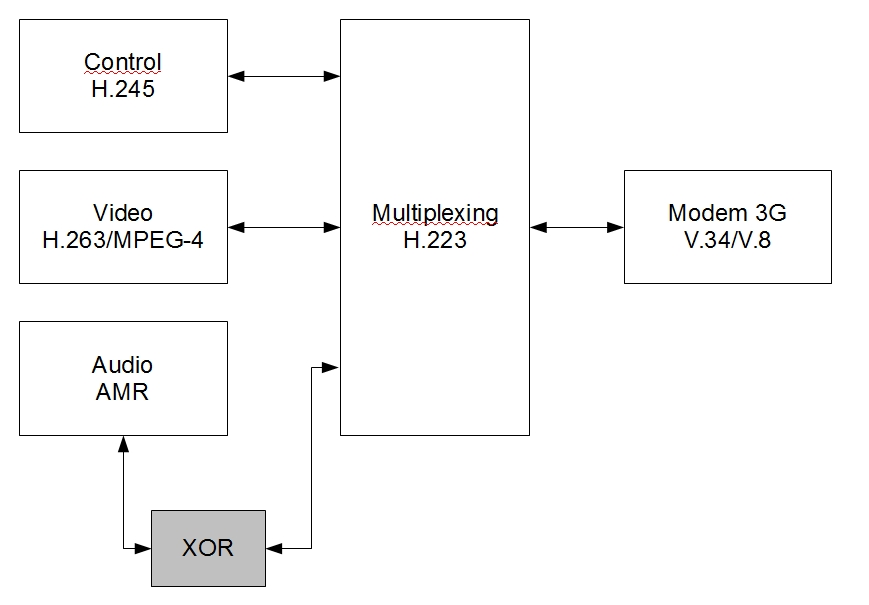
\includegraphics[scale=0.35]{pics/3g324m_template_bn.jpg}
%\caption{XOR-module}
%\label{fig:xor}
%\end{figure}

%\begin{figure}[!htbp]
%\centering
%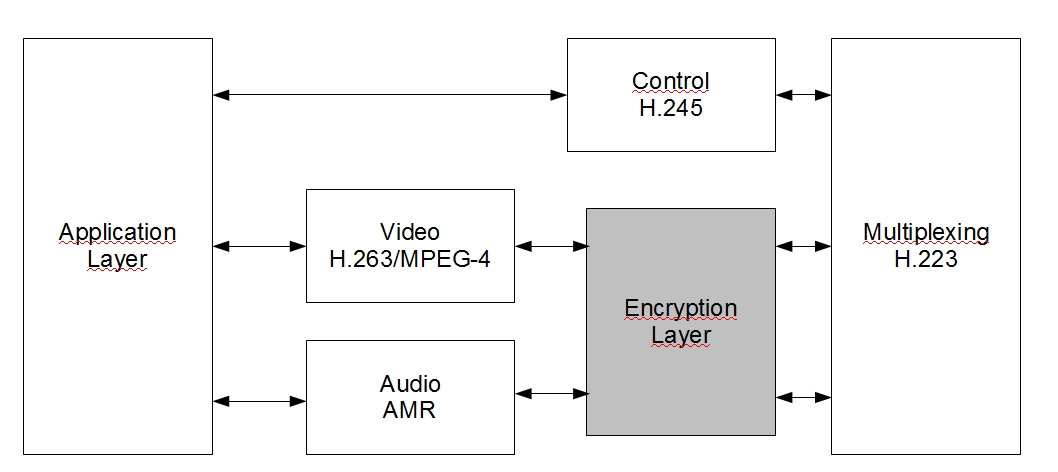
\includegraphics[scale=0.35]{pics/3g324m_encl.jpg}
%\caption{Encryption Layer}
%\label{fig:enc}
%\end{figure}

\subsubsection{Encryption Layer}
\label{EL}
%The EL described in Section \ref{EL} uses the cryptographic keys from a common pre-shared secret and do not perform any key-agreement or authentication protocol.
The EL is composed of two sub-modules which deal with the audio and the video streams. It implements AES to encrypt/decrypt the audio/video streams. On the transmitter, the audio sub-module takes the AMR audio as input and encrypts it using AES. The video sub-module runs a similar procedure encrypting the single blocks instead of the entire video frame, as discussed in Section~\ref{par:videocons}. On the receiver, the EL takes the encrypted packets coming from the multiplexing module as input and uses the appropriate key to decrypt them. The plain-text data is subsequently passed to the higher protocol layers.
\\
%\begin{figure}[!htbp]
%\centering
%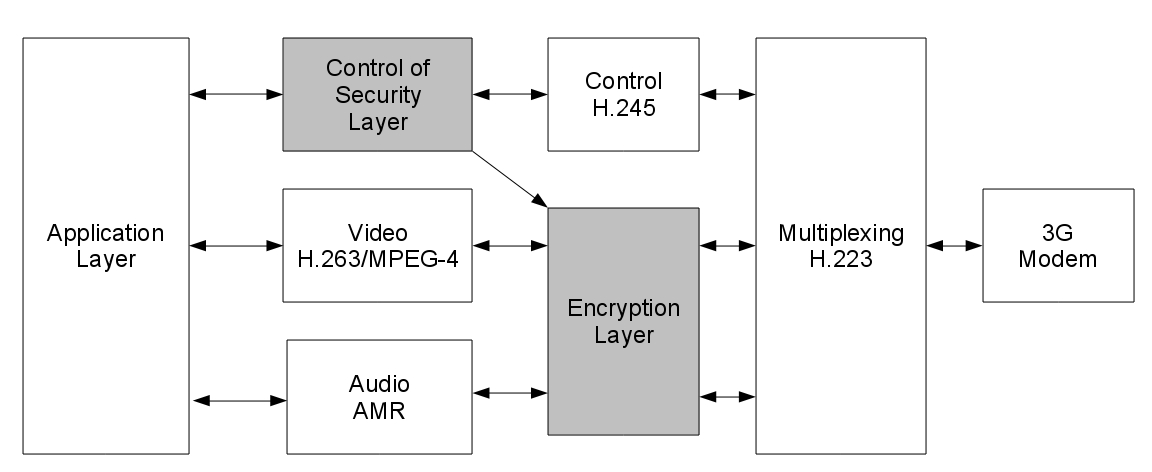
\includegraphics[scale=0.35]{pics/3g324m_template_fmw_bn.jpg}
%\caption{Control Layer}
%\label{fig:cl}
%\end{figure}

\subsubsection{Session Control Layer}
The SESCL is introduced in order to provide procedures to configure and manage the security mechanisms. As shown in Figure~\ref{fig:3g324sec}, it directly interacts with the AL and the EL.
The SESCL encapsulates the cryptographic protocols and performs all the session-specific operations as cryptographic keys management, EL initialization and virtual streams initialization. Simultaneously, it abstracts the AL from the underlying security protocols.
%With the introduction of the RTAL and the growing complexity of the cryptographic protocols implemented in SECR3T, the SCL became divided in two sub-layers: the previously described RTAL and the new SESCL. The overall SECR3T architecture is shown in Figure \ref{fig:3g324sec}.
It contains procedures to generate the cryptographic material used by the PBKDF2 function. Moreover, it provides a function to enable/disable on-the-fly the security extensions. This runtime activation function can be useful, for example, in order to avoid cryptographic overhead if encryption is not necessary.
\\

The SESCL includes robust well-known authentication and key-exchange protocols such as TLS and ECDH (see Section~\ref{par:authka} for details). It also provides primitives to integrate new communication protocols within the SECR3T system. In order to register a new protocol implementation, an adapter it is necessary which makes use of the RTAL functions (discussed below) to implement the communication between the peers. As a proof-of-concept, the SecIM protocol was implemented demonstrating the flexibility of the SCL managing general-purpose communication protocols.
\\

\subsubsection{Reliable Transport Adapter Layer}
Reliable data delivery is crucial for the proper functioning of the authentication and key-agreement protocols, because an error on a single bit during the data-exchange will cause the entire re-execution of the protocol. The extremely high BER of the wireless links ($ 10^{-3} \leq BER \leq 10^{-2} $) is worked around by implementing a reliable transport layer over the H.245 protocol.
%Cryptographic protocols must be implemented over a reliable transport layer, because the packet reception order and the guaranteed packet reception are crucial for their proper functioning.
%This work dealt with problems concerning very low (even though guaranteed) bandwidth constraints, extremely high bit error rate on wireless links ( $ 10^{-3} \leq BER \leq 10^{-2} $ ) and inflexible communication protocols. SECR3T worked around these issues implementing a reliable transport layer over the H.245 control protocol.
As explained in Section~\ref{par:3G324M}, H.245 provides reliable, acknowledged transmission of control information and segmentation of larger messages. Moreover, it provides support for user-defined communication through the \textit{UserInputIndication} message, originally introduced to simulate the transmission of DTMF tones over digital networks. In particular, the \textit{UserInputIndication} message is defined in the H.245 standard using the ASN.1 encoding and makes it possible to exchange arbitrary alphanumeric strings between the peers.
%\begin{figure}[!htbp]
%\centering
%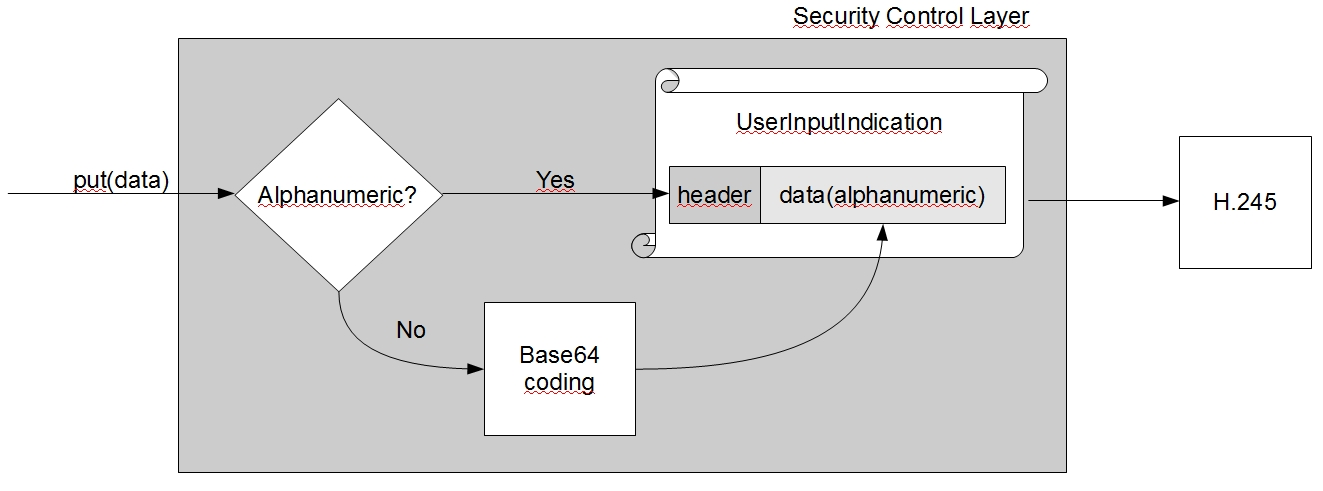
\includegraphics[scale=0.3]{pics/rtal_build_bn.jpg}
%\caption{Reliable Transport Adapter Layer - message transmission}
%\label{fig:rtal_snd}
%\end{figure}
The RTAL uses the \textit{UserInputIndication} mechanism to provide procedures in order to open virtual streams between the peers and transmit general-purpose data structures. The RTAL interface exposes a basic symmetric non-blocking primitive \emph{put()}, which sends data on an opened virtual stream, and a symmetric blocking primitive \emph{get()}, which receives data from an opened virtual stream.
%The Figure \ref{fig:rtal_snd} schematize the RTAL operation of sending data.

%As shown in Figure \ref{fig:rtal_snd}, the \emph{put()} function encapsulates a RTAL packet in an UserInputIndication message. The RTAL packet is firstly encoded in a base64-like alphanumeric string and encapsulated it into a H.245 compliant UserInputIndication message. The message transmission is completely demanded to the H.245 protocol, which guarantee the proper data delivery.

%On the other side (see Figure \ref{fig:rtal_rcv}), the receiver reads an opened virtual stream using the \emph{get()} function, which eventually waits until data reception. Incoming UserInputIndication messages are inspected and if a valid RTAL packet is found the reception procedure is called. It decodes the base64-like alphanumeric payload, reconstructs the original packet and returns the original data to the caller.

%\begin{figure}[!htbp]
%\centering
%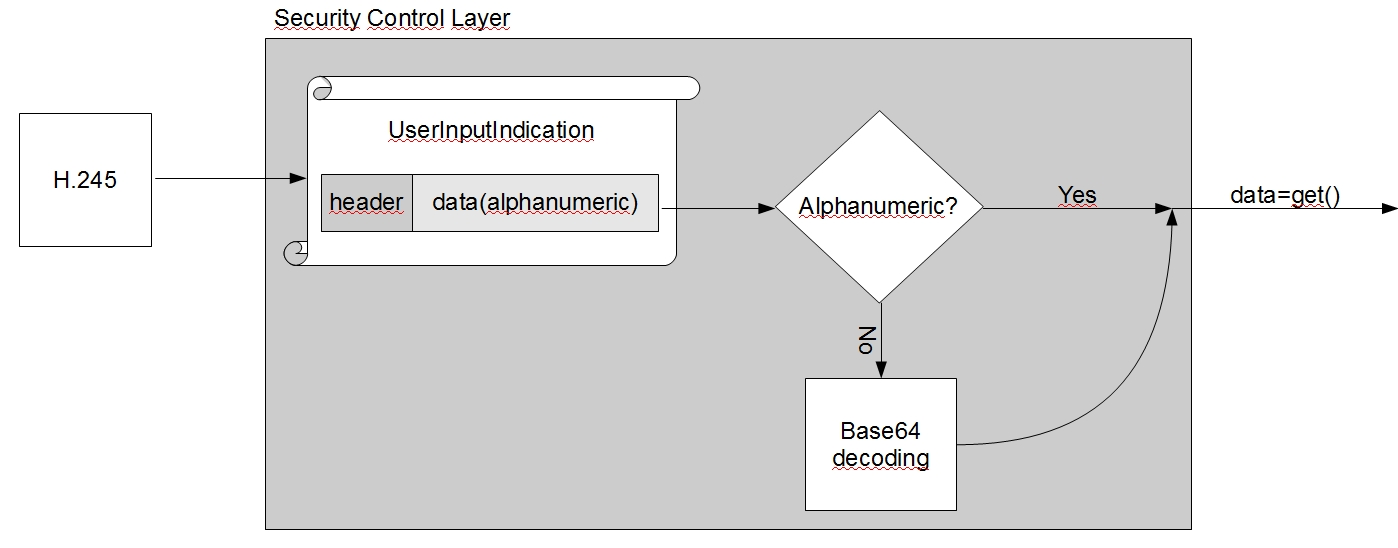
\includegraphics[scale=0.3]{pics/rtal_debuild_bn.jpg}
%\caption{Reliable Transport Adapter Layer - message reception}
%\label{fig:rtal_rcv}
%\end{figure}

%Contrary to multimedial communication protocols projected for IP networks, this work dealt with problems concerning very low (even though guaranteed) bandwidth constraints, extremely high bit error rate on wireless links ( $ 10^{-3} \leq BER \leq 10^{-2} $ ) and truly  inflexible communication protocols. We worked around these issues implementing a reliable transport layer over H.245 control protocol, in a similar but more flexible way of ITU-T H.235 recommendation: our project include the possibility of running and interchanging security protocols on-the-fly.

%\subsubsection{Authentication}

%The introduction of the RTAL opened the way to the implementation of a largest set of cryptographic protocols. In particular, the system includes some robust well-known authentication and key-exchange protocols as SSL and ECDH (see the Section \ref{par:design} for the specifications). To integrate an existing implementation of the SSL protocol, it is enough to create an adapter which instantiates the virtual streams through the RTAL functions and binds the imported I/O streams to the new ones.

%The integration of cryptographic protocols in SECR3T requires not big effort. In fact, thanks to the RTAL, an existing protocol implementation can be reused introducing a simple adapter layer which binds the imported I/O descriptors to the RTAL I/O functions. For example, to integrate an existing implementation of the SSL protocol, it is enough to create an adapter which instantiates virtual streams through the RTAL functions and binds the imported I/O streams to the created virtual streams. It is important to note that both the cryptographic protocol and the 3G-324M behavior are not affected by the SECR3T extension mechanism.

%\subsubsection{Session Control Layer}

%The SESCL is subsequently introduced to completely abstract the cryptographic protocols from the SECR3T system. It performs all the session-specific operations as cryptographic keys management, EL initialization, virtual streams initialization. At the same time, it abstracts the AL from the underlying authentication protocol.
%As shown in Figure \ref{fig:scl}, through the adapter is possible to \emph{register} a protocol at the SCL, and run it with a single procedure call.

%\begin{figure}[!htbp]
%\centering
%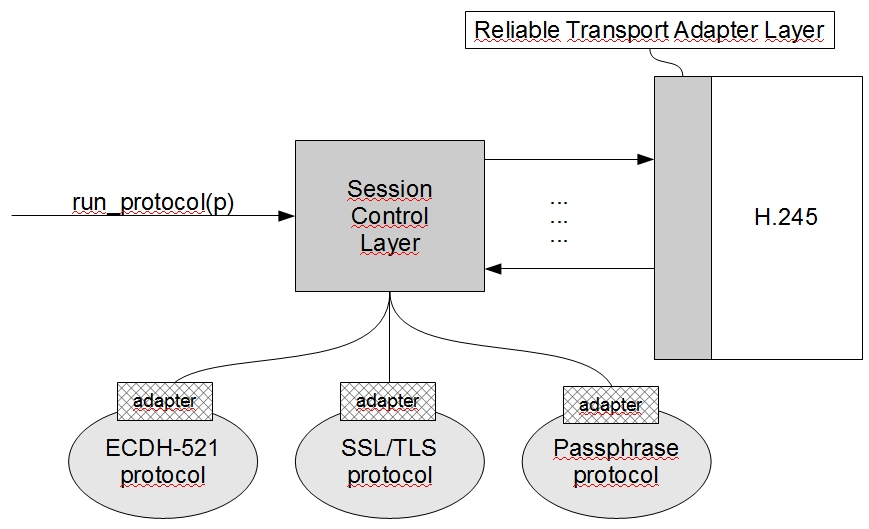
\includegraphics[scale=0.35]{pics/scllayer_bn.jpg}
%\caption{Session Control Layer}
%\label{fig:scl}
%\end{figure}

%With the introduction of the RTAL and the growing complexity of the cryptographic protocols implemented in SECR3T, the SCL became divided in two sub-layers: the previously described RTAL and the new SESCL. The overall SECR3T architecture is shown in Figure \ref{fig:3g324sec}.

%\begin{figure}[!htbp]
%\centering
%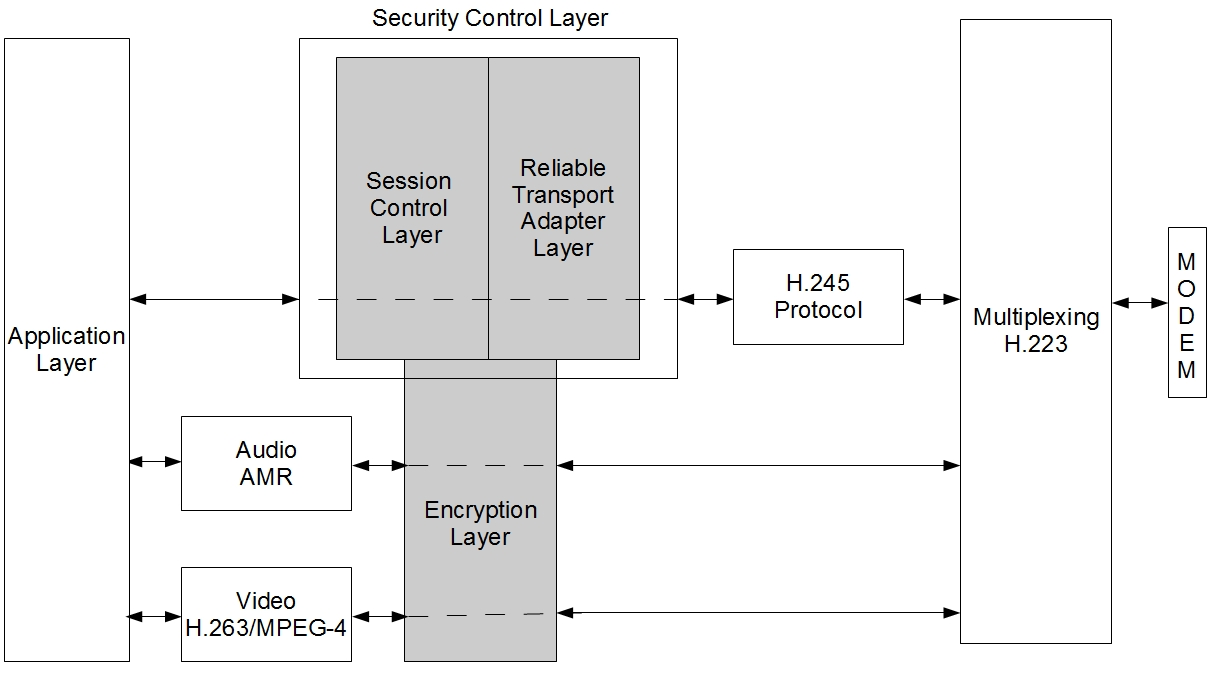
\includegraphics[scale=0.3]{pics/framework_bn.jpg}
%\caption{Overall SECR3T structure}
%\label{fig:fullfw}
%\end{figure}

%\subsubsection{Secure Instant Messaging protocol}
%
%A Secure Instant Messaging (SecIM) protocol has been also designed using the H.245 control channel. The SecIM protocol provides encryption and data integrity for textual messages. It demonstrates the flexibility of the RTAL managing general-purpose communication protocols.
%
%The SecIM protocol can be used during both secured and non-secured video-calls, without service interruption. It can be useful, for example, to communicate a credit card number, payment informations etc.


\subsection{Implemented protocol stack}

\begin{figure}[!htbp]
\centering
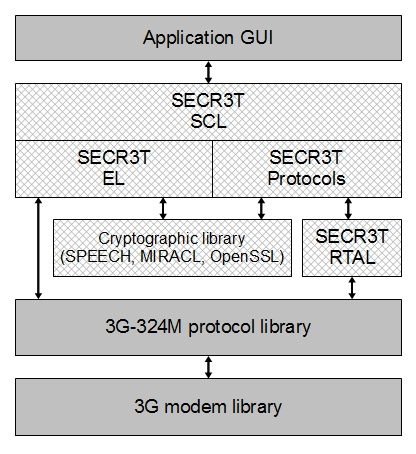
\includegraphics[scale=0.43]{pics/implementation_stack.jpg}
\caption{SECR3T implementation stack.}
\label{fig:implstack}
\end{figure}

A SECR3T prototype working in a real environment was developed by the authors.
%The 3G-324M protocol implementation and the videotelephony application have been provided by the Nexsoft company\cite{nexsoft}.
The prototype runs on PCs equipped with UMTS USB tokens and was implemented for Windows XP/7 platforms.

The overall implementation is in standard ANSI C++ and the adopted IDE was Visual Studio 2008. The project consists of more than three thousand source files and headers. OpenSSL was used to implement the TLS handshake. Implementations of ECDH, passphrase authentication and AES was imported from the SPEECH project, which uses the MIRACL\footnote{Multiprecision Integer and Rational Arithmetic C/C++ Library at~\url{http://www.shamus.ie/}} library for high-precision operations on elliptic curves.

Figure~\ref{fig:implstack} shows the SECR3T implementation stack. The users interact with the SECR3T GUI module, which sends commands to the SECR3T core modules. The SCL module manages the authentication and key-agreement procedures, and interacts with the EL, which creates the encrypted data channel. The data delivery is demanded to the 3G-324M protocol library, which directly interacts with the hardware.


%For these considerations, the overall SECR3T system is only dependant on the  implementation, and is easily portable if functions to intercept the audio/video traffic are provided.


\section{System performance}
\label{par:perf}
In order to gain a more detailed understanding of the impact produced by the proposed extension on the original 3G-324M protocol, an experimental analysis on the implemented prototype is required. Performance evaluation in this context is known to be difficult. This is mainly due to the unpredictable side-effects introduced by the network elements used to connect the endpoints. In fact, depending on the BS load and distance, the interconnection links can increase the system entropy. Consequently, the testing methodology is only aimed at measuring the effect introduced by the security modules/protocols on the overall system performances compared to the performances obtained using the standard (unencrypted) protocols.
%Whereas we are not concerned in channel bandwidth and reliability measurements.

Although an exhaustive performance analysis is not part of this study, the early experiments in a real environment have shown that the prototype is robust and flexible enough to be adopted under several network conditions. The key-agreement and authentication protocols were tested with success and the network never rejected the encrypted packets.

\subsection{Experimental setup}

In order to obtain factual results, SECR3T was tested using USIMs belonging to all the Italian UMTS network operators (TIM, Wind, Vodafone, H3G). The experiments were carried out using the 3G network as if regular customers. In other words, the operators were not aware of the tests being carried out.

The prototype was tested using the following hardware platforms:
\begin{itemize}
  \item PC1: Notebook with CPU Intel Core Duo T2300 at 1.66GHz, SDRAM DDR2 1GB;
  \item PC2: PC with CPU Intel Core Duo 2 E6400 at 2.13GHz, SDRAM DDR3 2GB.
\end{itemize}
The following devices were used for the 3G connectivity:
\begin{itemize}
  \item UMTS USB Token - Onda MSA523HS;
  \item UMTS USB Token - Onda MDC502HS.
\end{itemize}
The prototype was tested on Windows XP SP3 and Windows 7 Professional.

The execution time of the prototype procedures was measured using the high-resolution performance counter library, included in the Windows API, called \textit{QueryPerformanceCounter()}.


\subsection{Results}
\label{par:measure}
%The methodology adopted to measure the system performances rely on the key performance indicators discussed in Section~\ref{par:intro}.
The privacy provided by SECR3T to the user relies on the security strength of the cryptographic protocols that have been used.
The battery consumption strongly depends on the implementation of the adopted protocols. It was measured that a secure video-call, performing a TLS handshake and lasting 5 minutes, do not discharge the device battery more than 1/10 of the original video-call application.
The service quality was evaluated empirically, with the SECR3T implementation not showing to cause any detectable degradation of the user experience with respect to the ordinary video-call. The early experimental results were confirmed by an analysis of the delays introduced by the protocols and encryption procedures, respectively reported in Table~\ref{tab:delay_pp} and Table~\ref{tab:delay}.

\begin{table}[htbp]
\caption{Delay introduced by the protocol execution}
\centering

\begin{tabular}{| l | l | l |}
\hline
\textbf{Protocol} & \textbf{Minimum} & \textbf{Maximum}\\
\hline
Passphrase &  1678,73 msec & 2100,03 msec\\
\hline
ECDH & 1171,92 msec & 1363,27 msec\\
\hline
TLS & 6325,2 msec & 9227,11 msec \\
\hline

\end{tabular}

\label{tab:delay_pp}
\end{table}


\begin{table}[htbp]
\caption{Delay introduced by the local encryption procedures}
\centering

\begin{tabular}{ l | l | l |}
\cline{2-3}
& \multicolumn{2}{|c|}{\textbf{Data Type}}\\
\hline
\multicolumn{1}{|l|}{\textbf{Avg}} & \textbf{Audio} & \textbf{Video}\\
%\hline
%\textbf{Call duration} & 77 sec & 77 sec\\
%\hline
%\textbf{Number of packets} & 3756 & 1146\\
\hline
\multicolumn{1}{|l|}{\textbf{- per-packet delay}} & 0.00821606 ms & 0.0112831 ms\\
%\hline
%\textbf{Total delay} & 30.8595 ms & 12.9304 ms\\
\hline
\multicolumn{1}{|l|}{\textbf{- packets sent every 60sec}} & 3000 & 900 \\
\hline
\multicolumn{1}{|l|}{\textbf{- delay every 60sec}} & 24,65 ms & 10,15 ms\\
\hline
\end{tabular}

\label{tab:delay}
\end{table}


\section{Future works}
\label{par:future}

The experimental results of the SECR3T framework appear promising and encourage further research. In particular, the SECR3T project is a starting point to design mechanisms for the authenticity, integrity and non-repudiation of the conversation, in order to provide a multimedial communication service which has legal validity and can be used, for example, in a Court of Law for remote interrogations, in contracts signing, in remote purchases, etc.
\\

\noindent With this aim, the authors are working on the following improvements.
\\

\paragraph{User certificate in the USIM card}
The achieved implementation of the TLS protocol over 3G-324M for user-authentication and key-agreement is an important result and can motivate the introduction of digital certificates within USIMs, both simplifying and reinforcing the realized security infrastructure. However, this task should be implemented by the mobile telephone companies.
\\
%This work can also encourage the production of fully secured UMTS pendrives, providing secure telephony applications for voice, video, messaging and an encrypted filesystem to safely transport our personal data.

\paragraph{Audio/Video integrity}
A possible extension of SECR3T is the support for data integrity at the EL. This task may be difficult due to the inflexibility of the communication protocols. 
Audio and video packets have a fixed size, with it being possible to append information about data integrity (for example a HMAC code) only reducing the payload size.
This solution led to audio/video quality loss and is not compliant with the 3G-324M specifications.
A possible solution is to exploit the H.245 control channel to send the integrity information separately. However, it is important to note that audio/video packets are not numbered and packet loss is highly probable due to the BER, which increases the difficulty when implementing this solution.
\\

\paragraph{Non-repudiation}
%Mechanisms to guarantee the integrity and the authenticity of the overall conversation performed by the peers can be very useful. Behind these conditions, the peers can not repudiate their participation in the conversation and can not modify the conversation for own interest, therefore the saved conversation can have legal validity.

Non-repudiation mechanisms can be designed over the SECR3T framework. It would be useful for both parties to have, at the end of the communication, an identical copy of the conversation. Such a task is not easy as it seems because both the underlying communication channel and the transport protocol may be unreliable, with audio/video packets possibly being damaged or lost. The out-of-band H.245 channel could be used to implement this feature, for example, sending the digital signature and the integrity information of the packets.
%However, its implementation can be also hardened by the high BER which affects the wireless channels.

%\paragraph{Certificate storing.}
%Certificates store technique is not covered in this work.
%%, but an efficient solution to minimize communication overhead is proposed.
%An extended address book can be implemented associating public-keys to every known contacts in order to avoid full certificate retransmission, unless explicitly demanded by users.
%%Moreover, a standard compatible technique to insert the owner's picture within the certificates has been developed.

%\subsubsection{Performance improvements}
%The H.245 control channel represents a performance bottleneck due to its limited bandwidth. It is possible to speed up the protocol data transfers designing a reliable transport layer over the audio/video channels, which have more bandwidth with respect to the control channel.

\balance
\section{Conclusions}\label{par:conclusions}
%This research has shown that the 3G-324M protocol can be exploited to design a general-purpose communication channel over the proprietary telecommunication infrastructure. In particular, a large set of cryptographic end-to-end protocols can be implemented over the SECR3T framework.

This work demonstrates that it is possible to integrate cryptographic mechanisms within the 3G-324M protocol (and most generally in H.324) in a totally transparent way for the mobile operators, preserving compatibility with the 3G network specifications, resulting only in a minimal delay of the communication. The QoS provided by the telecommunication network for the underlying CS channel connecting the 3G-324M endpoints is generally better that the one provided for the IP channel in high mobility environments. The proposed solution is a valid alternative to the existing IP-based protocols for secure video-calling, providing reachability and availability features.

The SECR3T framework is an extended 3G-324M protocol which includes several security features. Authentication and key-agreement protocols were designed using the reliable H.245 control channel. The TLS handshake protocol provides strong user authentication using X.509 digital certificates. The SECR3T framework provides encryption for voice, video and textual communication. It supports the installation of new cryptographic protocols through its extensibility interface.

A SECR3T prototype was realized and tested in a real environment. Early experiments have confirmed the robustness of the SECR3T protocol. The TLS handshake takes between 8 and 13 seconds. The audio/video delay introduced by the encryption process is undetectable. Assuming that the user authentication only happens once at the beginning of the conversation, it is possible to conclude that the overall system performance seems to be suitable for real-case use. The authors are currently carrying out a detailed experimental analysis in order to minimize the impact of S3CRET on the overall system performance.


\bibliographystyle{IEEEtran}
\bibliography{3G-324M-Sec}


\end{document}
